\documentclass[12pt]{article}

\usepackage[utf8]{inputenc}
\usepackage{geometry}
\geometry{
    a4paper,
    total={170mm,257mm},
    left=25mm,
    right=25mm,
    top=25mm,
    bottom=25mm,
}
\usepackage{multicol}
\usepackage[font=small,labelfont=bf]{caption}
\setlength{\columnsep}{0.25cm}
\usepackage[inline]{enumitem}
\usepackage{amssymb}
\usepackage{xcolor}
\usepackage{mathtools} 
\setlength{\parindent}{0em}
\setlength{\parsep}{0em}
\usepackage{tikz}
\setlength{\parskip}{0em}
\usetikzlibrary{decorations.pathmorphing,patterns}
\usepackage[american,cuteinductors]{circuitikz}
\usetikzlibrary{shapes,arrows,circuits,calc,babel}
% Definition of blocks:
\tikzset{%
  block/.style    = {draw, thick, rectangle, minimum height = 3em,
    minimum width = 3em},
  sum/.style      = {draw, circle, node distance = 2cm}, % Adder
  input/.style    = {coordinate}, % Input
  output/.style   = {coordinate} % Output
}
% Defining string as labels of certain blocks.
\newcommand{\suma}{\Large$+$}
\newcommand{\inte}{$\displaystyle \int$}
\newcommand{\derv}{\huge$\frac{d}{dt}$}

\def\mf{\ensuremath\mathbf}
\def\mb{\ensuremath\mathbb}
\def\mc{\ensuremath\mathcal}
\def\lp{\ensuremath\left(}
\def\rp{\ensuremath\right)}
\def\lv{\ensuremath\left\lvert}
\def\rv{\ensuremath\right\rvert}
\def\lV{\ensuremath\left\lVert}
\def\rV{\ensuremath\right\rVert}
\def\lc{\ensuremath\left\{}
\def\rc{\ensuremath\right\}}
\def\ls{\ensuremath\left[}
\def\rs{\ensuremath\right]}
\def\bmx{\ensuremath\begin{bmatrix*}[r]}
\def\emx{\ensuremath\end{bmatrix*}}
\def\bmxc{\ensuremath\begin{bmatrix*}[c]}
\def\emxc{\ensuremath\end{bmatrix*}}
% \def\t{\lp t\rp}
% \def\k{\ls k\rs}

\newcommand{\demoex}[2]{\onslide<#1->\begin{color}{black!60} #2 \end{color}}
\newcommand{\demoexc}[3]{\onslide<#1->\begin{color}{#2} #3 \end{color}}
\newcommand{\anim}[3]{\onslide<#1->{\begin{color}{#2!60} #3 \end{color}}}
\newcommand{\ct}[1]{\lp #1\rp}
\newcommand{\dt}[1]{\ls #1\rs}

% \renewcommand{\familydefault}{\sfdefault}

\begin{document}
\begin{center}
\begin{large}
\textbf{Applied Linear Algebra in Data Analaysis}\\
\vspace{0.1cm}
\end{large}
\textbf{Linear Dynamical Systems \& Positive Definite Matrices Assignment}
\end{center}
\hrule
\vspace{1em}

\begin{large}
    \textbf{Marks: 26}
\end{large}

\begin{enumerate}
    \item Derive the state and measurement equations for the following composite systems, assuming the system $H_i$ to have the parameters $\ct{\mf{A}_i, \mf{B}_i, \mf{C}_i, \mf{D}_i}$. \textbf{[Marks: 6]}
    \begin{center}
        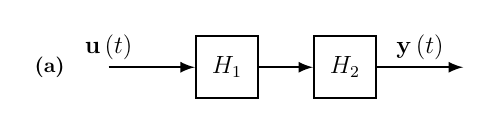
\begin{tikzpicture}[scale=0.75, transform shape, thick, node distance=2cm]
        \draw
            node [input, name=input1] {} 
            node [block, right of=input1] (sys1) {{\large $H_1$}}
            node [block, right of=sys1] (sys2) {{\large $H_2$}}
            node [input, right of=sys2, name=output1] {};
            \draw[-latex] node [above] {{\large $\mf{u}\ct{t}$}} (input1) -- node {} (sys1);
            \draw[-latex](sys1) -- node {} (sys2);
            \draw[-latex](sys2) -- node[above] {\large $\mf{y}\ct{t}$} (output1);
            \node[]  at (-1,0) {\textbf{(a)}};
        \end{tikzpicture}

        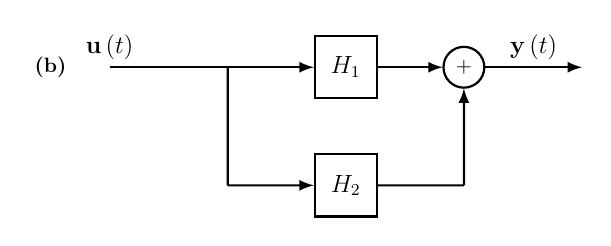
\begin{tikzpicture}[scale=0.75, transform shape, thick, node distance=2cm]
        \draw
            node [input, name=input1] {}
            node [input, right of=input1, name=tempin1] {} 
            node [input, below of=tempin1, name=tempin2] {} 
            node [block, right of=tempin1] (sys1) {{\large $H_1$}}
            node [block, right of=tempin2] (sys2) {{\large $H_2$}}
            node [sum, right of=sys1] (suma1) {$\suma$} 
            node [input, right of=sys2, name=tempout2] {}
            node [input, right of=suma1, name=output1] {};

            \draw[-] node [above] {{\large $\mf{u}\ct{t}$}} (input1) -- node {} (tempin1);
            \draw[-latex] node {} (tempin1) -- node {} (sys1);
            \draw[-] node {} (tempin1) -- node {} (tempin2);
            \draw[-latex] node {} (tempin2) -- node {} (sys2);
            \draw[-latex](sys1) -- (suma1);
            \draw[-] node {} (sys2) -- node {} (tempout2);
            \draw[-latex] node {} (tempout2) -- node {} (suma1);
            \draw[-latex] node {} (suma1) -- node[above] {\large $\mf{y}\ct{t}$} (output1);
            \node[]  at (-1,0) {\textbf{(b)}};
        \end{tikzpicture}

        \begin{tikzpicture}[scale=0.75, transform shape, thick, node distance=2cm]
        \draw
            node [input, name=input1] {}
            node [sum, right of=input1] (suma1) {$\suma$} 
            node [input, below of=suma1, name=tempfb] {} 
            node [block, right of=suma1] (sys1) {{\large $H_1$}}
            node [input, right of=sys1, name=tempout1] {}
            node [input, right of=tempout1, name=output1] {}
            node [input, below of=tempout1, name=tempout2] {}
            node [block, below of=sys1] (sys2) {{\large $H_2$}};

            \draw[-latex] node [above] {{\large $\mf{u}\ct{t}$}} (input1) -- node {} (suma1);
            \draw[-latex] node {} (suma1) -- node {} (sys1);
            \draw[-] node {} (sys1) -- node {} (tempout1);
            \draw[-latex] node {} (tempout1) -- node {} (output1);
            \draw[-] node {} (tempout1) -- node {} (tempout2);
            \draw[-latex] node {} (tempout2) -- node {} (sys2);
            \draw[-] node {} (sys2) -- node {} (tempin2);
            \draw[-latex] node {} (tempin2) -- node {} (suma1);
            \draw[-latex] node {} (tempout1) -- node[above] {\large $\mf{y}\ct{t}$} (output1);
            \node[]  at (-1,0) {\textbf{(c)}};
        \end{tikzpicture}
    \end{center}

    \item \textcolor{blue}{\textbf{[Programming]}} Write a python program to simulate a continuous-time mass, spring, damper system, described by the follloing differential equation.
    \[ M \ddot{y}(t) + B\dot{y}(t) + K y(t) = u(t) \]
    \textcolor{red}{Assuming the states of the system to be $\mf{x}\lp t \rp = \bmx y\lp t \rp \\ \dot{y}\lp t \rp \emx$, find out the matrices $\mf{A}, \mf{B}, \mf{C}, $ and $\mf{D}$.} \textbf{[Marks: 2]}

    Assuming that the input $u(t) = 0$, $\forall t \geq 0$, and assuming an initial condition of $\mf{x}\lp 0 \rp = \bmx 1 \\ 1\emx$, numerically solve the state compute the evolution of the state and the output of the system using the following procedure. Let $\Delta$ be the time step used for the integration, then the time is divided into discrete time instants $n \Delta$, where $n \in \mb{Z}_{\geq 0}$. Assuming that we know the value of the state at time $n\Delta$, the rate of change of the state $\dot{\mf{x}}$ and the output $\mf{y}\lp n\Delta \rp$ at a time $n \Delta$ are given by,
    \[ \begin{split}
        \dot{\mf{x}}( n \Delta ) &= \mf{A} \mf{x}(n \Delta) + \mf{B}\mf{u}(n \Delta) \\
        \dot{\mf{y}}( n \Delta ) &= \mf{C} \mf{x}(n \Delta) + \mf{D}\mf{u}(n \Delta)
        \end{split} \]
    We can compute the state at time $(n+1)\Delta$ from $\dot{\mf{x}}(n \Delta)$,
    \[ \mf{x}((n+1)\Delta) \approxeq \mf{x}\lp n\Delta\rp + \mf{x}\lp n\Delta \rp \cdot \Delta \]
    Starting from the value of the start at time $0$, $\mf{x}\lp 0 \rp$, we can numerically compute the evolution of the state for a given input $\mf{u}\lp t \rp$.

    \textcolor{red}{Compute the states and the output of the system from time $t = 0 s$ to $t = 10s$ for following values of the parameters $M, B, K$,} \textbf{[Marks: 3]}
    \textcolor{red}{\begin{enumerate}
        \item M = 1, B = 3, K = 1
        \item M = 1, B = 1, K = 1
        \item M = 0, B = 0, K = 1
    \end{enumerate}}

    \textcolor{red}{Carry out the simulations for different values of $\Delta = 0.1, 0.01, 0.001$. Compute the states and plot them as function of time.} \textbf{[Marks: 2]}

    \textcolor{red}{What differences do you find for the three systems for the different parameters and when using different step times? What do you think is the reason for the differences?} \textbf{[Marks: 2]}

    \item Prove that $\mf{A}^T\mf{A}$ is positive semi-definite for any matrix $\mf{A}$. When is $\mf{A}^T\mf{A}$ guaranteed to be positive definite? \textbf{[Marks: 2]}

    \item If $\mf{A}$ is positive definite, then prove that $\mf{A}^{-1}$ is also positive definite. \textbf{[Marks: 1]}

    \item Is the function $f\lp x_1, x_2, x_3\rp = 12 x_1^2 + x_2^2 + 6x_3^2 + x_1x_2 - 2x_2x_3 + 4x_3x_1$ positive definite?  \textbf{[Marks: 3]}
    
    \item Prove the following for $\mf{A} \in \mb{R}^{m \times n}$:  \textbf{[Marks: 4]}
    \[ \mf{A} = \bmx \mf{a}_1 & \mf{a}_2 & \ldots & \mf{a}_n\emx = \bmx \tilde{\mf{a}_1^T}\\ \tilde{\mf{a}_1^T} \\ \vdots \\ \tilde{\mf{a}_m^T}\emx \]
    \begin{enumerate}
        \item $\lV\mf{A}\rV_1 = \max_{1 \leq i \leq n} \lV\mf{a}_i\rV_1$
        \item $\lV\mf{A}\rV_\infty = \max_{1 \leq i \leq m} \lV\tilde{\mf{a}}_i\rV_1$
        \item $\lV\mf{A}\rV_2 = \max_{1 \leq i \leq n} \lv \lambda_i \rv$, where $\lambda_i$ are the eigenvalues of $\mf{A}^T\mf{A}$.
        \item $\lV\mf{A}\rV_F = trace\lp \mf{A}^T\mf{A}\rp$
    \end{enumerate}

    \item Prove that the induced norm of a matrix product is bounded:  \textbf{[Marks: 1]}
    \[ \lV\mf{A}\mf{B}\rV \leq \lV\mf{A}\rV\lV\mf{B}\rV \]

    \item Verify the following inequalities on vector and matrix norms ($\mf{x} \in \mb{R}^m$ and $\mf{A} \in \mb{R}^{m \times n}$):  \textbf{[Marks: 4]}
    \begin{enumerate}
        \item $\lV\mf{x}\rV_\infty \leq \lV\mf{x}\rV_2$
        \item $\lV\mf{x}\rV_2 \leq \sqrt{m}\lV\mf{x}\rV_\infty$
        \item $\lV\mf{A}\rV_\infty \leq \sqrt{n}\lV\mf{A}\rV_2$
        \item $\lV\mf{A}\rV_2 \leq \sqrt{m}\lV\mf{A}\rV_\infty$
    \end{enumerate}

\end{enumerate}

\end{document}